\section{Theorie}
\label{sec:Theorie}

\subsection{Der Glühelektrische Effekt}
\label{sec:glühelektr}
Ein Metall kann meist wie ein kristalliner Festkörper betrachtet werden.
Die ionisierten Leitungselektronen können sich im Inneren des Metalls recht frei
bewegen, da sie sich im Kraftfeld aller Ionen statt dem Kraftfeld eines Atoms
befinden. Ihre Beweglichkeit ähnelt den Molekülen innerhalb eines Gases.
Das Potential in dem sich die Leitungselektronen bewegen, kann in grober
Näherung als konstant betrachtet werden. Es unterscheidet sich von dem Potential
außerhalb des Metalls um den Betrag $\Phi$.
Um das Metall verlassen zu können, muss daher gegen ein Potential $\xi$ angelaufen
werden. Daraus ergibt sich eine zu leistende Austrittsarbeit von $e_0 \xi$,
wobei $e_0$ die Elementarladung bezeichnet.
Dieser Sachverhalt lässt sich gut mit einem Potentialtopf-Modell illustrieren:
\begin{figure}[H]
  \centering
  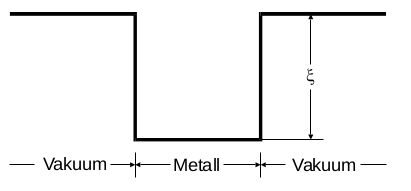
\includegraphics[scale=0.5]{content/potentialtopf.png}
  \caption{Potentialtopf-Modell eines Metalls. \cite{AP01}}
  \label{fig:potentialtopf}
\end{figure}
\noindent
Nach der Quantentheorie können die Elektronen nur diskrete Werte besitzen, welche
jedoch sehr nahe beieinanderliegen. Nach dem Pauli-Verbot kann jeder
mögliche Energiezustand nur von maximal zwei Elektronen mit entgegengestztem Spin
angenommen werden. Daher besitzen die Elektronen auch am absoluten Energienullpunkt
noch eine endliche Energie. Die Wahrscheinlichkeit, das ein Elektron eine bestimmte
Energie $E$ annimmt, wird durch die Fermi-Diracsche Verteilungsfunktion angegeben:
\begin{equation}
  f(E) = \frac{1}{e^{\frac{E - \xi}{k T}} + 1}.
  \label{eqn:fermidirac}
\end{equation}
\noindent
Hierbei bezeichnet $\xi$ die Fermische Grenzenergie, welche die Maximalenergie
der Elektronen bei $T = 0$ in Abhängigkeit der Zahl $n$ der Elektronen pro
Volumeneinheit des Metalls angibt. Bei Zimmertemperatur gilt für die Fermische
Grenzenergie $\xi >> kT$. Der Verlauf der Fermi-Dirac Verteilung ist folgender
Abbildung zu entnehmen:
\begin{figure}[H]
  \centering
  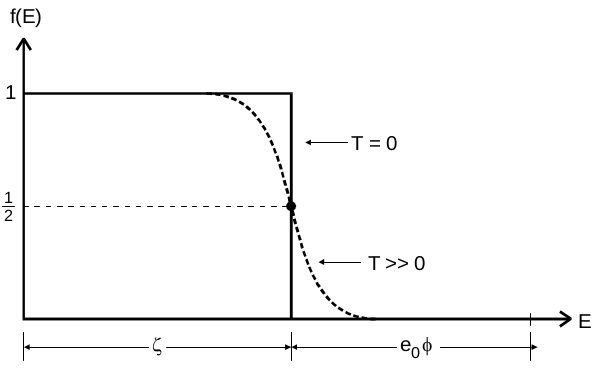
\includegraphics[scale=0.5]{content/fermidirac.png}
  \caption{Verlauf der Fermi-Dirac Verteilung. \cite{AP01}}
  \label{fig:fermidirac}
\end{figure}
\noindent
Ein Elektron benötigt daher zum Verlassen des Metalls eine Energie von
$\xi + e_0 \Phi$. Für diesen Wert gilt auch am Schmelzpunkt des Wolframs
$\xi + e_0 \Phi >> kT$. Aus diesem Grund kann für die Elektronen, welche
das Metall verlassen, die Gleichung \eqref{eqn:fermidirac} durch Folgende
angenähert werden:
\begin{equation}
  \centering
  f(E) \approx e^{\frac{\xi -E}{kt}}.
  \label{eqn:approxfermidirac}
\end{equation}
\noindent

\subsection{Die Sättigungsstromdichte}
\label{sec:sättstromd}
Die Sättigungsstromdichte beschreibt die Anzahl der Elektronen, die pro Zeiteinheit
und Flächeneinheit aus der Metalloberfläche heraustreten in Abhängigkeit von
der Temperatur. Hierfür wird ein Koordinatensystem mit Z-Achse orthogonal zu der
Metalloberfläche eingeführt. Mithilfe von Gleichung \eqref{eqn:approxfermidirac}
sowie der Anzahl $d\alpha$ der Elektronen aus dem Volumenelement des Impulsraumes
kann gezeigt werden, das folgendes gilt:
\begin{equation}
    d\alpha = \frac{\partial E}{\partial p_z} n(E) dp_x dp_y
    dp_z = n(E) dE dp_x dp_y dp_z.
    \label{eqn:elektronenvolumenelement}
\end{equation}
Hierbei beschreibt $n(E)$ die Zahl der Elektronen pro Volumeneinheit ihres
Phasenraumes. Hier kann verwendet werden, dass jeder Quantenzustand im Phasenraum
das Volumen $h^3$ einnimmt, woraus folgt:
\begin{equation}
    n(E) = \frac{2}{h^3}f(E).
    \label{eqn:anzahlelektronen}
\end{equation}
Hierbei beschreibt $f(E)$ die Wahrscheinlichkeit, mit der ein zur Energie $E$
gehörendes Element des Phasenraumes besetzt ist.
Aus Gleichung \eqref{eqn:elektronenvolumenelement} und \eqref{eqn:anzahlelektronen}
ergibt sich, dass nur die Elektronen die Metalloberfläche verlassen können, für
die gilt:
\begin{equation}
    \frac{p_z^2}{2 m_0} > \xi + e_0 \Phi.
    \label{eqn:elektronengeschwkomponente}
\end{equation}
Die Sättigungsstromdichte ergibt sich nun durch Abzählen aller Elektronen,
deren Geschwindigkeitskomponente in $z$-Richtung Gleichung
\eqref{eqn:elektronengeschwkomponente} erfüllen. Dieser Wert muss dann mit $e_0$
multipliziert werden. Hierraus folgt die Richardson-Gleichung:
\begin{equation}
    j_s(T) = 4 \pi \frac{e_0 m_0 k^2}{h^3}T^2 \text{exp}\left(\frac{-e_0 \Phi}{k T}\right).
    \label{eqn:richardson}
\end{equation}

\subsection{Die Hochvakuum-Diode}
\label{sec:hochvak}
Um den in Abschnitt \ref{sec:sättstromd} beschriebenen Sättigungstrom, der aus
einer Metalloberfläche emittiert wird, messen zu können, muss ein Hochvakuum
vorliegen, weil die Wechselwirkungen der freien Elektronen mit einem Gas die
Messung unmöglich machen würden. Ebenfalls wird ein elektrisches Feld benötigt,
welches die emittierten Elektronen absaugt. Daher wird in einem evakuierten
Glaskörper mit einem darin eingeschmolzenen Draht einen Strom an diesen Draht angelegt,
sodass dieser auf Temperaturen zwischen $1000 \si{\kelvin}$ bis $3000 \si{\kelvin}$
erhitzt werden kann. Gegenüber dieser Kathode steht eine Anode, welche die aus
dem Draht austretenden Elektronen absaugt. Diese Apparatur wird als
Hochvakuum-Diode bezeichnet. Sie ist in folgender Abbildung dargestellt.
\begin{figure}[H]
  \centering
  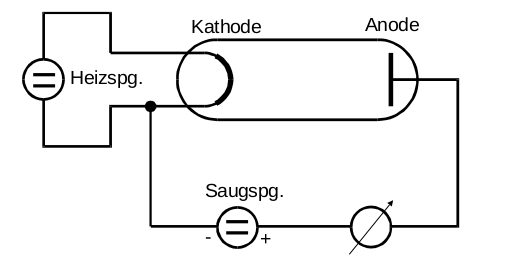
\includegraphics[scale=0.5]{content/hochvakuumdiode.png}
  \label{fig:hochvakuumd}
  \caption{Schematische Darstellung einer Hochvakuum-Diode. \cite{AP01}}
\end{figure}
\noindent
Für die Heizleistung der Kathode gilt folgende Relation:
\begin{equation}
  I_f U_f = f \eta \sigma T^4 + N_{WL}.
  \label{eqn:heizleistung}
\end{equation}
Hierbei meint $\sigma = 5.1 \cdot 10^{-12}\si{\watt\per\centi\meter\squared\kelvin^4}$
die Stefan-Boltzmannsche Strahlungskonstante, $f$ die emittierende Kathodenoberfläche
sowie $\eta = 0.28$ den Emissionsgrad der Oberfläche.

\subsection{Die Langmuir-Schottkysche Raumladungsgleichung}
\label{sec:langmuirschottky}
Der Strom, welcher zu der Anode fließt, ist abhängig von der angelegten
Anodenspannung. Wenn diese zu niedrig ist, kann es passieren, dass nicht alle
von der Diode emittierten Elektronen die Anode erreichen. Bei höheren Strömen
kann eine Unabhängigkeit des Anodenstroms von der Anodenspannung erreicht werden.
Da die Elektronen auf die Anode zu beschleunigt werden, gilt auch für niedrige
Spannungen das Ohmsche Gesetz nicht. Aufgrund dieser Tatsache ist die
Raumladungsdichte $\rho$ der Elektronen abhängig von dem Ort, sie nimmt zu der
Anode hin ab. Für die Stromdichte $j$ gilt nach der Kontinuitätsbedingung, dass
sie konstant ist. Zwischen $j$ und $\rho$ gilt jedoch folgende Relation:
\begin{equation}
  j = -\rho v.
  \label{eqn:anodenstromdichte}
\end{equation}
Daraus folgt, dass $\rho$ den Verlauf der Feldstärke zwischen Anode und Kathode
beeinflusst. Das Feld der Anode wird abgeschirmt. Aus diesem Grund ist der
gemessene Diodenstrom kleiner als nach Gleichung \eqref{eqn:richardson} zu
erwarten wäre.
Um einen quantitativen Zusammenhang zu erhalten, wird mit der Potentialgleichung
begonnen:
\begin{equation}
  \Delta V = -\frac{1}{\epsilon_0} \rho.
  \label{eqn:Potentialgleichung}
\end{equation}
Nun wird die Vereinfachung vorgenommen, dass Anode und Kathode unendlich ausgedehnt
sind und sich in einem festen Abstand gegenüberstehen. Dann sind $V$ und $\rho$
nur von der Ortskoordinate $x$ abhängig. Mithilfe von Gleichung
\eqref{eqn:richardson} und Gleichung \eqref{eqn:anodenstromdichte} sowie dem
Energiesatz $e_0 V = \frac{m_0}{2} v^2$ ergibt sich
\begin{equation}
  \sqrt[4]{V^3(x)} = \frac{3}{4} \sqrt{\frac{4 j}{\epsilon_0 \sqrt{2 e_0/m_0}}}x.
  \label{eqn:gleichung11}
\end{equation}
Also wächst das Potential nach einem $\sqrt[3]{x^4}$-Gesetz. Die Feldstärke
wächst daher nach einen $x^{\frac{1}{3}}$-Gesetz und $\rho$ proportional zu
$x^{-\frac{2}{3}}$. Dies ist in folgender Abbildung dargestellt.
\begin{figure}[H]
  \centering
  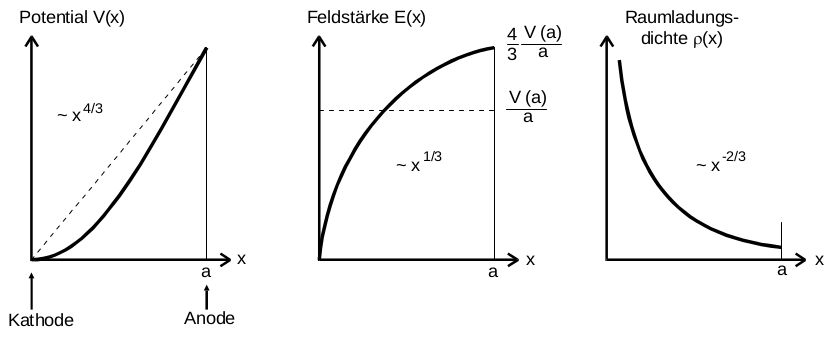
\includegraphics[scale=0.5]{content/langmuirschottky.png}
  \label{fig:langmuirschottky1}
  \caption{Die Ortsabhängigkeit des Potentials, der Feldstärke und der
  Raumladungsdichte im Raumladungsgebiet einer Hochvakuumdiode. \cite{AP01}}
\end{figure}
\noindent
Für die Raumladungsdichte gilt nun das Langmuir-Schottkysche Raumladungsgesetz:
\begin{equation}
  j = \frac{4}{9} \epsilon_0 \sqrt{2 e_0/m_0} \frac{V^{3/2}}{a^2}.
  \label{eqn:langmuirschottky2}
\end{equation}
An \eqref{eqn:langmuirschottky2} ist erkennbar, dass $j$ hier mit
$V^{\frac{3}{2}}$ wächst.

\subsection{Das Anlaufstromgebiet der Hochvakuumdiode}
Entgegen Gleichung \eqref{eqn:gleichung11} wird auch bei $V = 0$ ein
geringer Anodenstrom gemessen. Der Anodenstrom entsteht hier durch die
Eigengeschwindigkeit der Elektronen. Nach Gleichung \eqref{eqn:fermidirac} gibt
es eine endliche Anzahl an Elektronen, die bei $T = 0$ eine Energie besitzen,
die größer als die Austrittsarbeit ist. Der hierraus resultierenden
Energieüberschuss kann als kinetische Energie der Elektronen gemessen werden.
Der Energieüberschuss beträgt
\begin{equation}
  \Delta E = E - (\xi + e_0 \Phi).
  \label{eqn:energieübersch}
\end{equation}
Aufgrund dieser Energie können die Elektronen auch ein geringes Gegenfeld
überwinden. Aufgrund dieser Tatsache wird dieser Strom auch als
Anlaufstrom bezeichnet. Auch die Anode besitzt eine Austrittsarbeit $\Phi_A$, diese ist
jedoch größer als die der Kathode. Durch die elektrisch leitende Verbindung
zwischen Anode und Kathode außerhalb der Diode werden die Fermi-Oberflächen
(d.h. die Stelle E = \xi auf der Energieachse) der Metalle auf die gleiche Höhe
gebracht. Daher werden sie mit einem äußeren Potential $V$ um $e_0 V$
gegeneinander verschoben. Dies ist in folgender Abbildung dargestellt.
\begin{figure}[H]
  \centering
  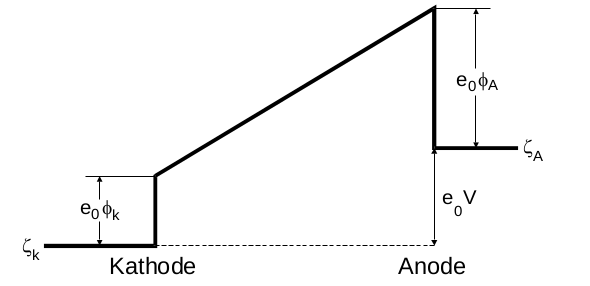
\includegraphics[scale=0.5]{content/anlaufstrompot.png}
  \caption{Die Potentialverhältnisse im Anlaufstromgebiet der Diode. \cite{AP01}}
  \label{fig:anlaufstrompot}
\end{figure}
\noindent
Daher besitzen diejenigen Elektronen, welche die Anode erreichen, eine Energie
$E > e_0 \Phi + e_0 V$. Die Zahl der Leitungselektronen mit einer Energie zwischen
$E$ und $E + dE$ kann durch folgende Gleichung angenähert werden:
\begin{align}
  j(V) & = j_0 \cdot \text{exp}\left(-\frac{e_0 \Phi_A + e_0 V}{kT}\right) \\
       & = \text{const} \cdot  \text{exp}\left(-\frac{e_0 V}{kT}\right).     \\
  \label{eqn:anlaufstrom}
\end{align}

\subsection{Die Kennlinie der Hochvakuumdiode}
Die Kennlinie einer Hochvakuumdiode gliedert sich in drei Abschnitte. Der erste
Abschnitt heißt Anlaufstromgebiet und zeichnet sich durch einen exponentiellen
Zusammenhang zwischen $I$ und $V$ aus. Das Anlaufstromgebiet liegt bei $V < 0$.
An das Anlaufstromgebiet schließt sich das Raumladungsgebiet an, in dem eine
$\sqrt{V^3}$-Abhängigkeit vorliegt. Daran schließt sich das Sättigungsstromgebiet
an, da das Raumladungsgesetz nicht für unbegrenzt hohe Anodenspannungen gültig ist.
Eine solche Kennlinie einer Hochvakuumdiode ist in folgender Abbildung dargestellt.
\begin{figure}[H]
  \centering
  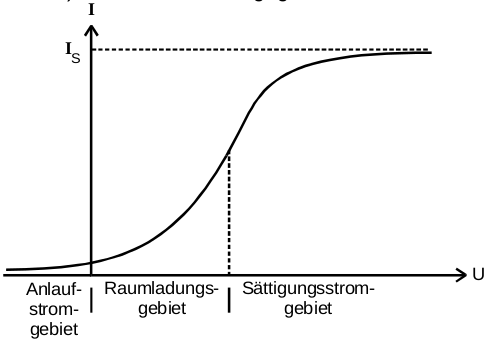
\includegraphics[scale=0.5]{content/kennlinie.png}
  \label{fig:kennlinie}
  \caption{Die Kennlinie einer Hochvakuumdiode. \cite{AP01}}
\end{figure}
